\documentclass[hidelinks,a4paper,12pt]{article}
\addtolength{\oddsidemargin}{-1.cm}
\addtolength{\textwidth}{2cm}
\addtolength{\topmargin}{-2cm}
\addtolength{\textheight}{3.5cm}
\newcommand{\HRule}{\rule{\linewidth}{0.5mm}}
\makeindex

\usepackage{longtable}
\usepackage[pdftex]{graphicx}
\usepackage{makeidx}
\usepackage{hyperref}
\hypersetup{
	colorlinks=true,
	linkcolor=black,
	filecolor=magenta,      
	urlcolor=cyan,
}


% define the title
\author{Men-at-Work}
\title{ Software Requirements Specification}
\begin{document}
	\setlength{\parskip}{6pt}
	
	% generates the title
	\begin{titlepage}
		
		\begin{center}
			% Upper part of the page       
			
\includegraphics[width=1\textwidth]{./Graphs/UPLogo2012.jpg}\\[0.4cm]    
			\textsc{\LARGE Department of Computer Science}\\[1.5cm]
			\textsc{\Large COS 301 - Software Engineering}\\[0.5cm]
			% Title
			\HRule \\[0.4cm]
			%%
\includegraphics[width=0.05\textwidth]{./logo.png}\\[0.4cm] 
			{ \huge \bfseries Software Requirements Specification}\\[0.4cm]
			\HRule \\[0.4cm]
			% Author and supervisor
			\begin{minipage}{0.4\textwidth}
				\begin{flushleft} \large
					\emph{Authors:}
				\end{flushleft}
			\end{minipage}
			\begin{minipage}{0.4\textwidth}
				\begin{flushright} \large
					\emph{Student number:}
				\end{flushright}
			\end{minipage}
			
			\begin{minipage}{0.4\textwidth}
				\begin{flushleft} \large
					Muller {Potgieter}
				\end{flushleft}
			\end{minipage}
			\begin{minipage}{0.4\textwidth}
				\begin{flushright} \large
					\emph{}
					u12003672
				\end{flushright}
			\end{minipage}
			
			\begin{minipage}{0.4\textwidth}
				\begin{flushleft} \large
					Sara {Masilela}
				\end{flushleft}
			\end{minipage}
			\begin{minipage}{0.4\textwidth}
				\begin{flushright} \large
					\emph{}
					u10126202
				\end{flushright}
			\end{minipage}
			
			\begin{minipage}{0.4\textwidth}
				\begin{flushleft} \large
					Lethabo {Mogase}
				\end{flushleft}
			\end{minipage}
			\begin{minipage}{0.4\textwidth}
				\begin{flushright} \large
					\emph{}
					u14103207
				\end{flushright}
			\end{minipage}
			
			\begin{minipage}{0.4\textwidth}
				\begin{flushleft} \large
					Stuart {Andrews}
				\end{flushleft}
			\end{minipage}
			\begin{minipage}{0.4\textwidth}
				\begin{flushright} \large
					\emph{}
					u12153983
				\end{flushright}
			\end{minipage}
			
			\begin{minipage}{0.4\textwidth}
				\begin{flushleft} \large
					Stephen {Swanepoel}
				\end{flushleft}
			\end{minipage}
			\begin{minipage}{0.4\textwidth}
				\begin{flushright} \large
					\emph{}
					u11032091
				\end{flushright}
			\end{minipage}
			
			\begin{minipage}{0.4\textwidth}
				\begin{flushleft} \large
					Renton {Mclntyre}
				\end{flushleft}
				\end{minipage}
				\begin{minipage}{0.4\textwidth}
				\begin{flushright} \large
				\emph{}
				u14312710
				\end{flushright}
			\end{minipage}
			
			\begin{minipage}{0.4\textwidth}
				\begin{flushleft} \large
					Sibusiso {Masemola}
				\end{flushleft}
			\end{minipage}
			\begin{minipage}{0.4\textwidth}
				\begin{flushright} \large
					\emph{}
					u12270467
				\end{flushright}
			\end{minipage}

			
			\vfill
			% Bottom of the page
			{\large \today}
		\end{center}
	\end{titlepage}
	\footnotesize
	%\input{declaration_of_originality.tex}
	\normalsize
	
	
	\pagenumbering{roman}
	\tableofcontents
	\newpage
	\pagenumbering{arabic}
	
	\newpage
	\section{Introduction} This section deals with the software software requirements specification of the program. This includes:
	\begin{itemize} 
		\item The vision.
		\item The background.
		\item The access channel requirements.
		\item The quality requirements.
		\item The integration requirements.
		\item The architecture requirements.
		\item Use cases.
		\item Required functionality.
	\end{itemize}
	
	\section{Vision}
	The client wishes to create a program that allows users to keep track of their own work, as well as collaborate with other users, so that they can write papers together. Users will be able to specify the progress that they have made with their papers and alter them as needed. The program will keep a full record of all changes made to the papers, in order to create a time line of events. The program will be available as a desktop and mobile application, as well as being available as a web version.
	
	\section{Background}
	\begin{enumerate}
		\item A specialized program, aimed at research papers does not exist that is not indigenous to the UP CS department
		\item It can be used as a common platform for researchers around the world to easily manage their work and collaborate more easily
		\item It will allow researchers easier access to their work and provides access to domain objects
		\item It will allow researchers to keep track of their progress more easily
		\item The program can be expanded to include researchers from other universities or scientific bodies
	\end{enumerate}
	\newpage
	
	\section{Architecture Requirements}
	\subsection{Access Channel Requirements}
	\begin{enumerate}
		\item A desktop application available in the form of a Windows (7/8/10) client, a Linux client and binaries
		ready to be built on either system with an interactive GUI
		\item A web version compatible with all major browsers (eg. Mozilla Firefox, Google Chrome or Opera)
		\item A mobile application developed for Android and compatible with all current and upcoming versions thereof
	\end{enumerate}
	
	This will be accomplished by making use of RESTful web services (these being based on the REST, or REpresentational State Transfer architecture). The system itself will accept HTTP requests from any of these channels
	and create responses in the form of JSON strings, a format easily handled in any one of the aforementioned access
	systems.
	Additionally, the following access channels can be added:
	\begin{enumerate}
		\item A command line (terminal) based version of the desktop application, which could be suitable for the target
		audience, who are very technologically capable
		ready to be built on either system with an interactive GUI
		\item A mobile application developed for Windows Phone and/or iOS.
	\end{enumerate}
	
	\subsection{Quality Requirements}
	The following assurances must be made in terms of quality:
	\begin{itemize}
		\item Performance
		\begin{enumerate}
			\item The server must always provide the minimum data required to fulfill a request. That is to say, were a user to log in to the system, the server should only send the data pertaining to that user to be displayed, no papers related to his/her co-authors or other related parties. 
			\item The system must be created with the most minimal and efficient coding practices possible, given that the result must still be reliable and robust.
			\item No actual files are to be stored in the system, lest it negatively affect the performance components of the system itself.
		\end{enumerate}
		\item Reliability
		\begin{enumerate}
			\item The system must be thoroughly tested on both the client and server side, to ensure it will not cause faults or problems. It is important that no data is lost, thus the coding used to create the system must be defensive and thorough.
		\end{enumerate}
		\newpage
		\item Scalability
		\begin{enumerate}
			\item The system must be designed such that:
			\newline
	 a - The client is able to handle and display details of a large, potentially infinite number of Publications.\newline
				b - The server is able to handle, display details pertaining to large, potentially infinite number of Users, Authors and Publications.	
			\item Modular programming should be used in order to ensure that there are no restrictions in terms of the system's ability to be extended and improved upon at later stages.
		\end{enumerate}
		\item Security
		\begin{enumerate}
			\item It should not be possible for individuals other than the actual Users to access or modify the system. This means that security has to be ensured in terms of password storage, secure login methods and user management (methods such as re-obtaining password via email should be very carefully guarded).
			\item It should not be possible for Users to make changes to other Users' details, as it is with non-User Authors, unless they are one of a select few Super Users or Administrators.
			\item A publication should not be able to be removed from a system, only edited, unless it is removed by an aforementioned Super User.
			\item A User should not be capable of viewing or editing a publication for which they are not on the list of Authors.
		\end{enumerate}
		\item Flexibility
		\begin{enumerate}
			\item The system should be capable of reacting quickly to different stimuli. This means (as an example) that if multiple users are concurrently using the system and performing vastly differing tasks which make use of completely different parts of the same system, there should not be any noticeable loss of performance.
			\item The system should be able to perform well even under bulk loads, without loss of data on the way.
			\item It should be possible to add new components or fields to existing components in the system without making major changes. 
		\end{enumerate}
		\item Maintainability
		\begin{enumerate}
			\item The system should be developed with current and maintained technologies, so as to avoid loss of support for as long as possible.
			\item The system should be well documented so as to ensure future developers on the system are capable of maintaining the system without worry.
			\item When changes are made in current technologies, the system should be updated as soon as possible to reflect relevant changes.
			\item The modular design of the system must be such that if changes must be made to a part of the system, only that part itself should be changed.
		\end{enumerate}
		\item Monitorability 
		\begin{enumerate}
			\item All actions taken that have any affect on the databases stored server side are to be logged.
			\item All logs, current connections and current activity must be viewable by the Super Users in charge of the system.
		\end{enumerate}
		\item Integrability
		\begin{enumerate}
			\item The system should be designed in such a manner (with modularity and common interfacing methods) that it is capable of having pieces or services plugged in and catered to with minimal effort, such as e-mail notification, which could be a logical future addition to the system for the sake of deadline maintenance.
		\end{enumerate}
		\item Cost
		\begin{enumerate}
			\item The tools used to design the system should, as far as possible be open source, free and not require a license.
			\item In certain cases, paid and licensed software may be suitable for some individual pieces of the system, such as having a Database Management System (DBMS) to handle the storage of data as best possible.
			\item Costs may be created in the form of external hosting for the web service and database storage, should the client desire it to be so.
		\end{enumerate}
		\item Usability
		\begin{enumerate}
			\item The Users, being staff members, must have easy access from any channel.
			\item The system should be designed in such a manner that the interface is easy to learn and use.
			\item The system should be minimal and avoid having unnecessary visuals that could impair a User's ability to use the system comfortably.
		\end{enumerate}
	\end{itemize}
	
	
	\subsection{Integration Requirements}
	
	Given that the system in question is intended to use external systems to as minimal a degree as is possible, this section will instead be dedicated to the explanation behind why focusing on Integration Requirements is in fact a detrimental procedure to this project plan.
	
	\begin{enumerate}
		\item Firstly, it should be noted that this is a private system. This means that there is little need for a connection with any system which provides linkage to a major network of users.
		\item The system itself is simplistic and requires no extra functionality provided by more complex external systems, as it is capable of functioning aptly with simplistic HTTP requests and a simple Object Data Type for communication. Although this could be stretched to CORBA at a later stage and thus require some management of this system, as the system currently stands, it is sufficient to use basic JSON strings and work with these.
		\item The system is personal to the degree that one may not view more than one's own profile. This implies that it would be redundant to make use of extra technologies, in a system which at its core is just a very small database management tool, with access only to one's own part of a database.
	\end{enumerate}
	Regarding the future, it is important to note that the system is intended to be modular and adaptable, thus it could (possibly) be integrated into an external, or vice versa. The focus of such an endeavor would be on ensuring this does not compromise the system in any way. To guard against this, we must ensure the following:
	\begin{enumerate}
		\item The system is not dramatically affected by the changes made, in terms of performance. That is to say, given a new, external system being integrated into the existing system (such as e-mail notification), there should not be any noticeable performance drops that would hinder usage, as this would be detrimental to the system and possibly be a good reason to not perform such integrations in the first place.
		\item The system is not to be compromised in terms of security. An example of this would be if an external system attempted to send or receive secure data via insecure means (eg. requiring raw, unencrypted data that should be sensitive).
		\item It  should still be possible to accurately monitor all external systems that are integrated with the original system.
		\item The external system used should not be relied on too heavily by the original system, unless adequate reliability and safety redundancies can be assured.
		\item The external system should not compromise the ability of the original system to be used in a scalable manner (that is to say, it should not make it less efficient or plausible to use the system for larger volumes of data or users).
	\end{enumerate}
	With this in mind, the final note on this topic is as follows: 
	\begin{enumerate}
		\item The protocols and systems used along with the original system that is to be created should never be overly complex or dramatic. 
		\item The system should, as a whole, remain independent and capable of being used in a modular and free manner. 
		\item An over reliance on external systems should be avoided and the integration between systems must be fluid and as loosely coupled as possible.
	\end{enumerate}
	
	\subsection{Architecture Constrains}
			\subsubsection{ Since the system will be web-based, technologies that guide in building web pages will be needed, i.e.:}
		
		\begin{itemize} 
			\item HTML 5
			\newline
			This is the overall language that will be used to develop the layout and functionality of the web page
				\item Bootstrap
				\newline
			This technology will be used to style the web page. Styling with this technology will reduce the work load giving us more time to work on the 				functionality of the system.
				\item Apache
				\newline
			We will use this as reference to how the final product will look, since we won’t have access to the client’s server until the system is completed.	
				\item jQuery and Java Script
				\newline
			These two languages will be used for client side validation, i.e. validation of user credentials upon logging in to the system.	
				\item PHP
				\newline
			PHP will be used for validation on the server side.	
				\item SQL
				\newline  
			This technology will be used to enter information to the database. Entries will be stored separately:
			Users,
			Authors and Co-Authors
		\end{itemize}
		
		
		The system will also have an Android application version. The technologies that will be used are:
			\begin{itemize} 
		\item Android Studios
		\newline
		This will be the main technology used to build the main functionality of the system.
		
		\item Programming languages like Java, C++ and C will be used to assist in building the Android version of the system  
		\end{itemize} 
		
		\subsubsection{ Architecture Patterns / Framework }
		
		The application will make use of a four-tier layered pattern, which consists of:
	
	\begin{enumerate} 
			\item The Presentation layer
			\newline
		This layer consists of an interface through which the users can access the application layer. This 	layer also captures the user's input, validates it and passes the information to the application 	layer.
		
			\item The Application layer 
			\newline
		This layer provides the back-end services of the system, i.e. the functionality of the system. 	Access to the web services layer is managed in this layer. The application layer may also be 	used as temporary storage when the database cannot be accessed.
		
			\item The Web Services layer
			\newline
		Here the information that was processed in the application layer is received and passed 	down to the database. Access to the database will be read and write. This layer is where the 	sever is situated.
		
			\item The Data layer
			\newline
		This layer is the actual database. The information is added to the database in this layer.
	\end{enumerate}
	
	\section{Functional Requirements and application design}
	\subsection{ Use Case Prioritization}
	
	
	\begin{enumerate}
		
		\item  User Login -- Critical.
		
		\item  Author Login -- Important.
		
		\item  Super-user Login -- Critical.
		
		\item  User registration -- Critical.
		
		\item  Author registration -- Important.
		
		\item  Super-user Registration -- Critical.
		
		\item  Creating a User -- Critical.
		
		\item  Creating an Author -- Important.
		
		\item  Creating a new publication -- Critical.
		
		\item  Editing a publication -- Nice-to-Have
		
		\item  Setting the status of a publication -- Important.
		
		\item  Viewing Publications as an Author -- Nice-to-Have.
	\end{enumerate}
	
	\noindent 
	
	
	\subsection{ Use case/Services contracts}
	
	\begin{enumerate}
		\item  User Login
		
		\begin{enumerate}
			\item  Pre-Conditions
			
			\begin{enumerate}
				\item  A user must be registered as a user by admin before he/she is able to login to the Research Paper App.
				
				\item  In order to login a user must enter in his/her correct authentication details.
			\end{enumerate}
			
			\item  Post-Conditions
			
			\begin{enumerate}
				\item  The user has access to his/her profile and publications.
				
				\item  The user may alter his/her publications.
				
				\item  The user may access only his/her profile and publications and no others.
				
				\item  A user can be an author.
			\end{enumerate}
		\end{enumerate}
		
		\noindent 
		
		\item  Author Login
		
		\begin{enumerate}
			\item  Pre-Conditions
			
			\begin{enumerate}
				\item  An author must be registered by admin as an author before he/she may login to the Research Paper App.
				
				\item  In order for an author to login he/she must enter in his/her correct authentication details
			\end{enumerate}
			
			\item  Post-Conditions
			
			\begin{enumerate}
				\item  The author has access to any profile that he/she co-authored.
				
				\item  The author may not alter any publications that he/she was involved in.
				
				\item  A user can be an author, but an author cannot be a user.
			\end{enumerate}
		\end{enumerate}
		
		\noindent  
		
		\item  Super-user/admin Login
		
		\begin{enumerate}
			\item  Pre-Conditions
			
			\begin{enumerate}
				\item  A single user must be able to logon as admin or a super user.
				
				\item  In order to login a user must enter in his/her correct authentication details.
			\end{enumerate}
			
			\item  Post-Conditions
			
			\begin{enumerate}
				\item  The super-user has access to any and all user and author profiles.
				
				\item  The super-user is the only user capable of adding more users and authors.
				
				\item  The super-user can alter any profile.
			\end{enumerate}
		\end{enumerate}
		
		\noindent  
		
		\item  User Registration
		
		\begin{enumerate}
			\item  Pre-Conditions
			
			\begin{enumerate}
				\item  The admin or super-user is in charge of registering the users.
			\end{enumerate}
			
			\item  Post-Conditions
			
			\begin{enumerate}
				\item  The user receives his/her login details.
				
				\item  The user has his/her privileges set.
				
				\item  The user is registered in the user and author database tables.
				
				\item  The user is able to logon to the Research Paper App with the login details supplied by the super-user/admin.
			\end{enumerate}
		\end{enumerate}
		
		\noindent  
		
		
		\item  Author Registration
		
		\begin{enumerate}
			\item  Pre-Conditions
			
			\begin{enumerate}
				\item  The admin or super-user is in charge of registering the authors.
			\end{enumerate}
			
			\item  Post-Conditions
			
			\begin{enumerate}
				\item  The author receives his/her login details.
				
				\item  The author has his/her privileges set.
				
				\item  The author is registered in the author database table only.
				
				\item  The author is able to logon to the Research Paper App, as an author, with the login details supplied by admin or super-user.
			\end{enumerate}
		\end{enumerate}
		
		\noindent  
		
		\item  Super-user/Admin Registration
		
		\begin{enumerate}
			\item  Pre-Conditions
			
			\begin{enumerate}
				\item  Upon system-initialization, a single user sets him/herself to the super-user/admin.
				
				\item  This user uses his/her authentication details to log in as the super-user/admin.
			\end{enumerate}
			
			\item  Post-Conditions
			
			\begin{enumerate}
				\item  The super-user/admin can add and remove users
				
				\item  The super-user/admin can view all user and author profiles, as well as lists of publications associated with each.
			\end{enumerate}
		\end{enumerate}
		
		\noindent  
		
		\item  Creating a User
		
		\begin{enumerate}
			\item  Pre-Conditions
			
			\begin{enumerate}
				\item  Prior to a user logging into his/her profile, the super-user/admin must have created the user profile, which the user logs onto.
				
				\item  Upon logging in, a user must have full access to his/her profile page.
				
				\item  Profile page must include
				
				\begin{enumerate}
					\item  Full name of user.
					
					\item  Contact details
					
					\item  Cell phone number.
					
					\item  Telephone number.
					
					\item  Email Address.
					
					\item  Conference for whom the user is researching.
					
					\item  List of links to publications.
					
					\item  A list of co-authors per publication (if any).
				\end{enumerate}
			\end{enumerate}
			
			\item  Post-Conditions
			
			\begin{enumerate}
				\item  The user must be able to edit his/her publication list as he/she sees fit.
				
				\begin{enumerate}
					\item  Adding Publications.
					
					\item  Removing Publications.
				\end{enumerate}
				
				\item  The user may only view/edit his/her own profile and publications.
			\end{enumerate}
		\end{enumerate}
		\noindent 
		
		\item  Creating an Author: Use Case Prioritization -- Important
		
		\begin{enumerate}
			\item  Pre-Conditions
			
			\begin{enumerate}
				\item  Prior to the author logging into his/her profile the super-user/admin must assign him/her an author profile.
				
				\item  Upon logging in, the author must have full access to his/her profile.
			\end{enumerate}
			
			\item  Post-Conditions
			
			\begin{enumerate}
				\item  Authors may not alter publications.
				
				\item  Displayed on their profile will be:
				
				\begin{enumerate}
					\item  Full name of the author.
					
					\item  Contact details
					
					\item  Cell phone number.
					
					\item  Telephone number.
					
					\item  Email Address.
				\end{enumerate}
				
				\item  Authors will be able to see each of the publications that they co-authored.
				
				\begin{enumerate}
					\item  No altering will be allowed. 
				\end{enumerate}
			\end{enumerate}
		\end{enumerate}
		
		\noindent 
		
		
		\item  Creating a new publication:
		
		\begin{enumerate}
			\item  Pre-Conditions
			
			\begin{enumerate}
				\item  The user or super-user must provide a publication title.
				
				\item  The supervisor of the paper must be included.
				
				\item  All the authors who worked under that supervisor, to co-author the paper, must be listed.
				
				\item  A deadline must be set.
				
				\item  Progress of the paper must be specified.
				
				\begin{enumerate}
					\item  Ongoing.
					
					\item  Terminated.
					
					\item  Completed.
				\end{enumerate}
			\end{enumerate}
			
			\item  Post-Conditions
			
			\begin{enumerate}
				\item  The new publication will be viewable by the user, the super-user and all authors involved.
				
				\item  The publication may only be edited by the user who created the publication, or the super-user.
			\end{enumerate}
		\end{enumerate}
		
		\noindent  
		
		\item  Editing a publication
		
		\begin{enumerate}
			\item  Pre-Conditions
			
			\begin{enumerate}
				\item  User or super-user must first successfully log on.
				
				\item  Only the user who is the supervisor or owner of the paper may edit the publication.
				\begin{itemize}
					\item An author who happens to be a user as well as an author may not edit another user’s publication.
				\end{itemize}
				
				\item  The super-user/admin may edit any profiles publication he/she wants.
			\end{enumerate}
			
			\item  Post-Conditions
			
			\begin{enumerate}
				\item  The user or the super-user/admin can alter the following:
				
				\begin{enumerate}
					\item  The Author list,
					
					\item  The status of the paper,
					
					\item  The deadline of the paper,
					
					\item  The name of the paper,
				\end{enumerate}
				
				\item  Or remove the publication all together.
			\end{enumerate}
		\end{enumerate}
		
		\noindent 
		
		\noindent 
		
		\item  Setting the status of a publication
		
		\begin{enumerate}
			\item  Pre-Conditions
			
			\begin{enumerate}
				\item  If a user has successfully logged on, then he/she may view and alter the publications.
			\end{enumerate}
			
			\item  Post-Conditions
			
			\begin{enumerate}
				\item  Depending upon the status of the paper the user may alter it.
				
				\item  Only a user, whose privileges allow it, may edit the publication. 
			\end{enumerate}
		\end{enumerate}
		
		\noindent  
		
		\item  Viewing Publications As an Author
		
		\begin{enumerate}
			\item  Pre-Conditions
			
			\begin{enumerate}
				\item  Upon logging in, the author must have full access to his/her profile.
				
				\item  Profile page must include
				
				\begin{enumerate}
					\item  Full name of user.
					
					\item  Contact details
					
					\item  Cell phone number.
					
					\item  Telephone number.
					
					\item  Email Address.
					
					\item  Supervisor who the author is researching under.
					
					\item  List of links to publications for which he/she has co-authored.
				\end{enumerate}
			\end{enumerate}
			
			\item  Post-Conditions
			
			\begin{enumerate}
				\item  All publications that the author has co-authored must be available to view.
				
				\item  Unless the author is also a user, he/she will be prohibited from altering any data  
			\end{enumerate}
		\end{enumerate}
	\end{enumerate}
	
	
	
	\begin{itemize}
		\item  Request and Results Data Structures
	\end{itemize}
	
	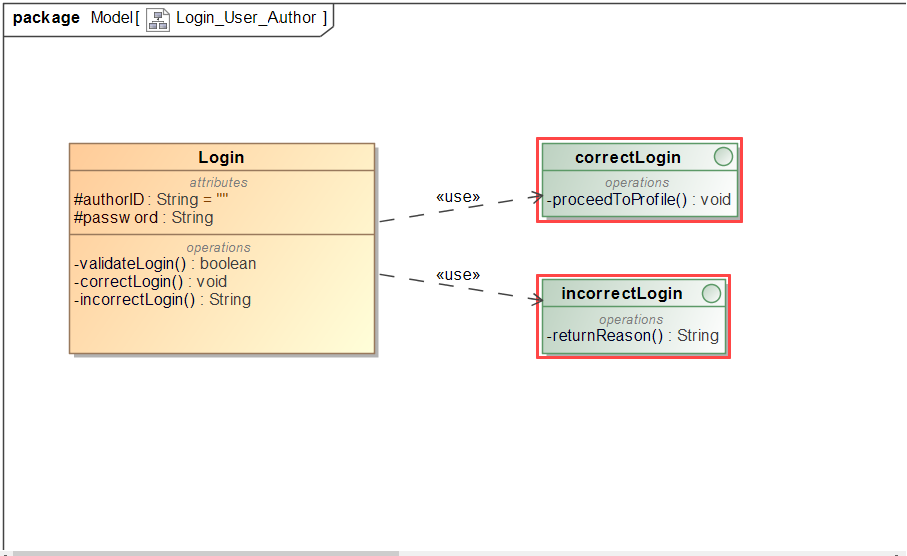
\includegraphics[width=1\textwidth]{./Graphs/Login.png}\\[0.4cm]  
	
	Figure 5.2.1: Login for Author and User.
	
	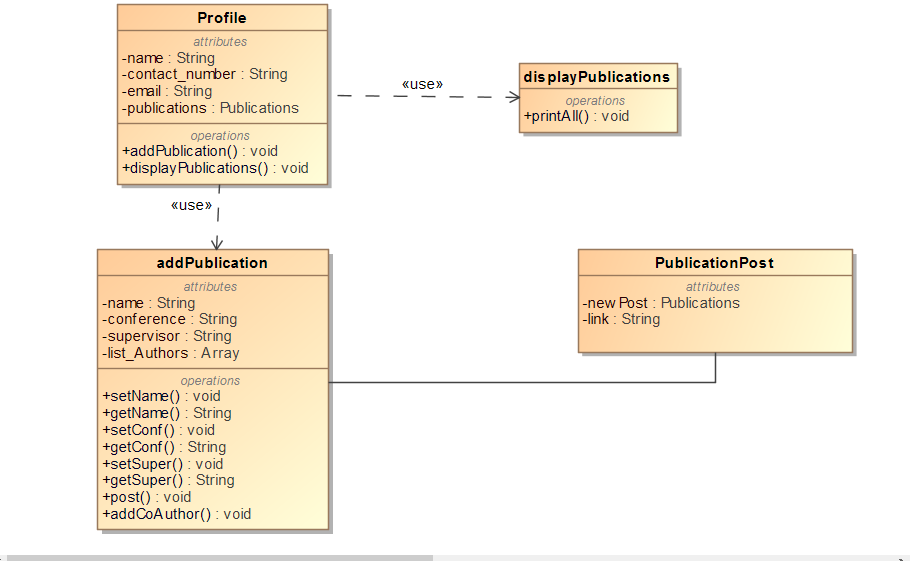
\includegraphics[width=1\textwidth]{./Graphs/Posting.png}\\[0.4cm]  
	
	Figure 5.2.2: User posting publication.
	
	
	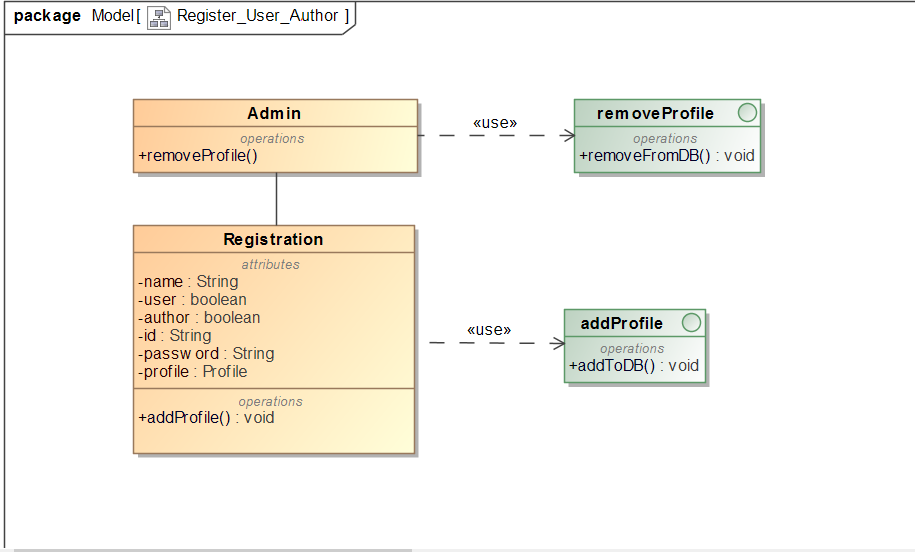
\includegraphics[width=1\textwidth]{./Graphs/Registration.png}\\[0.4cm]  
	Figure 5.2.3: Registration
	
	\subsection{Functionality Requirements}
	\subsubsection{Server Functional Requirements}
	
	%%5.3.1.1 Connection
	\subsubsection{Connection}
	
	This connection provides communication between client, server     
	and the relational database, achieving this through a 	protocol 
	that allows multiple access (<100) to the server, at 	one time.
	\begin{itemize}
		\item A client is able to log in a request 
		
		\item A client is able to send a request which goes through the server 	to the database.
		
		\item Conversion of request to a database query is performed.      	
	\end{itemize}
	
	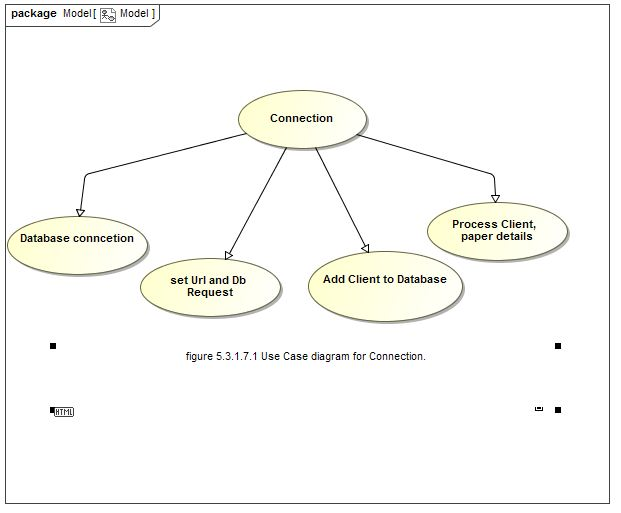
\includegraphics[width=1\textwidth]{./Graphs/UseCaseforConnection.JPG}\\[0.4cm]  
	Figure 5.3.2: Connection
	
	\subsubsection{Database Connection}
	
	Server must be connected to database, every time it is in use. 
	No information is left on server and not recorded on database.  
	
	\begin{itemize}
			\item Database is accessible any time by server, on client request. 
	\end{itemize}
	
	
		\subsubsection{Send paper to browser client}
	
	Sending paper to browser, provides a requested paper data to the  
	web browser. It is a step by step process
	
	\begin{itemize}
	\item Perform validation on whether the paper exists in the database.
	\item Retrieves the paper from the database, to server, to web browser
\end{itemize}

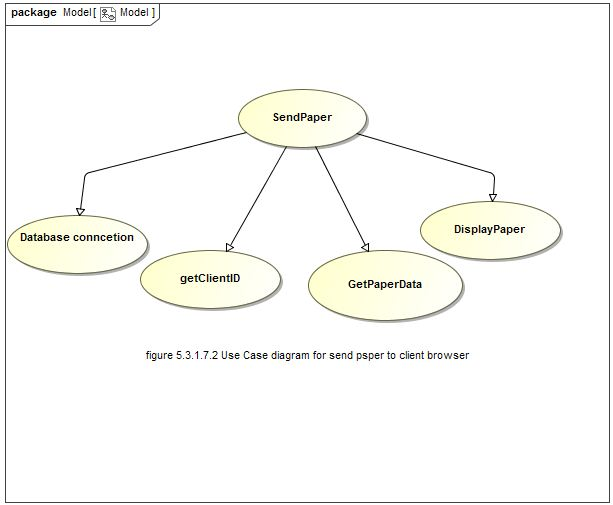
\includegraphics[width=1\textwidth]{./Graphs/UseCaseforSendPaper.JPG}\\[0.4cm]  
Figure 5.3.3: Send Paper
	
		\subsubsection{Get paper from browser client}
	
	This process provides receiving paper data from the browser client,
	This is a result of “pushing” the paper data to the database after    
	it has been edited. 
	
		\begin{itemize}
			\item Perform validation on paper if it is recent.(date modified).
			\item Replace paper data on the database, with the new one.
		\end{itemize}
		
		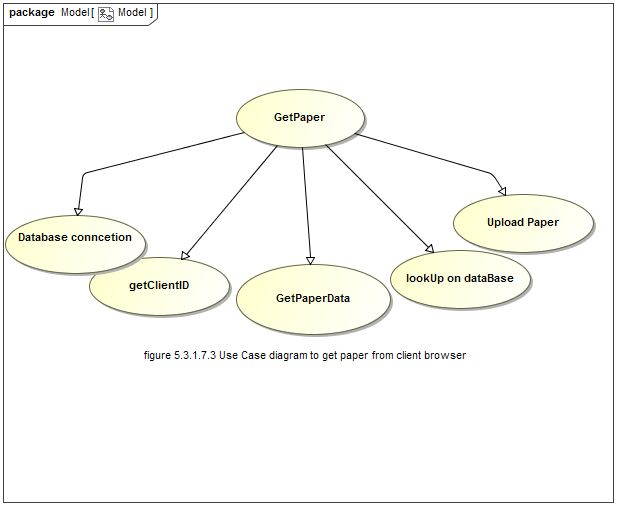
\includegraphics[width=1\textwidth]{./Graphs/UseCaseforGetpaper.JPG}\\[0.4cm]
		Figure 5.3.4: Get Paper
	
	\subsubsection{Send Author list to browser client}
	
	Providing the list of authors in the system. Results in a navigable
	list.		
	
	\begin{itemize}
		\item Get all authors from the database, to the server, to the client browser.
		\item Allow viewing to navigate through authors.
	\end{itemize}
	
	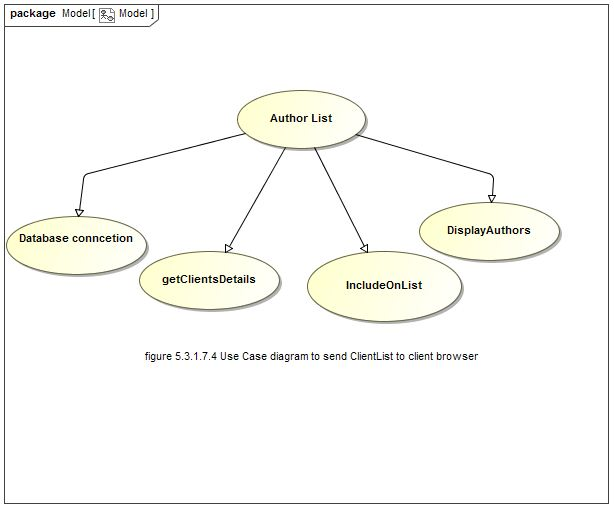
\includegraphics[width=1\textwidth]{./Graphs/UseCaseforAuthorList.JPG}\\[0.4cm]
	
	5.3.5 Send Client List
	 
	
		\subsubsection{User Identification}
	
	User Identification provides the means to get client (user) credentials and log them in the system to their appropriate profile. 
	
	\begin{itemize}
		\item User name of the client(client browser)
		\item User password of the client (client browser)
		\item Validate with users in database. 
	\end{itemize}
	
	
	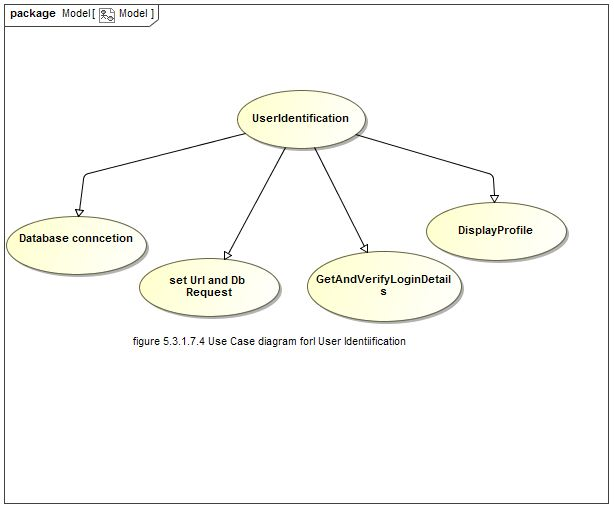
\includegraphics[width=1\textwidth]{./Graphs/UseCaseforUserIdentification.JPG}\\[0.4cm]
	Figure 5.3.6 User Identification
	
	\subsubsection{Process Specifications}
	
	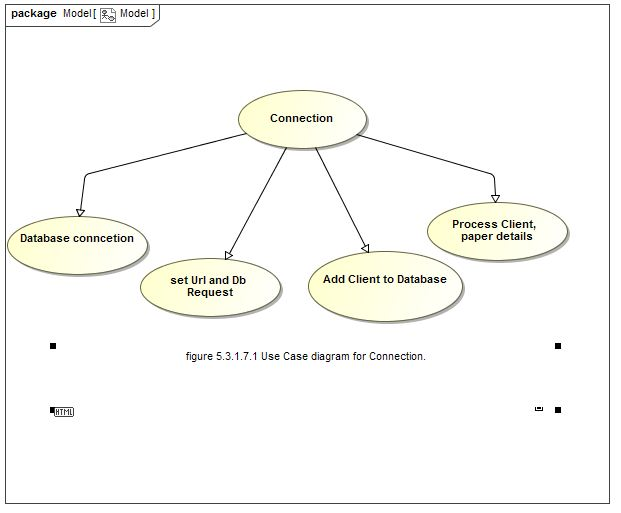
\includegraphics[width=1\textwidth]{./Graphs/UseCaseforConnection.jpg}\\[0.4cm]
	
		Figure 5.3.6: Connection
		

	\subsubsection{Browser Client Functional requirements}
		
		\subsubsection{Log in to server}
		
		Log in allows user (client browser) to log in to the system, resulting 
		in their profile information and current work loaded on the browser.  
		
		\begin{itemize}
			\item Enter their username
			\item Enter their password
		\end{itemize}
		
			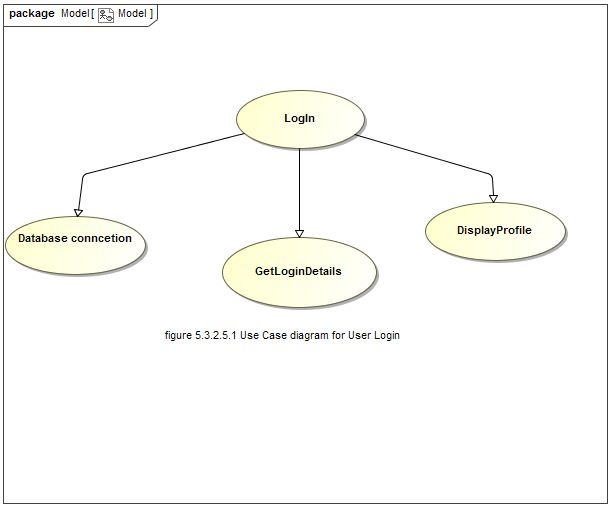
\includegraphics[width=1\textwidth]{./Graphs/UseCaseforLogIn.JPG}\\[0.4cm]
			Figure 5.3.7: Log In
		
		\subsubsection{Locate paper data}
		
		Loads paper upon selection/request from the system, as the user (client)  
		may be involved in multiple papers. Upon request the server will load 
		correct paper data. 
		
			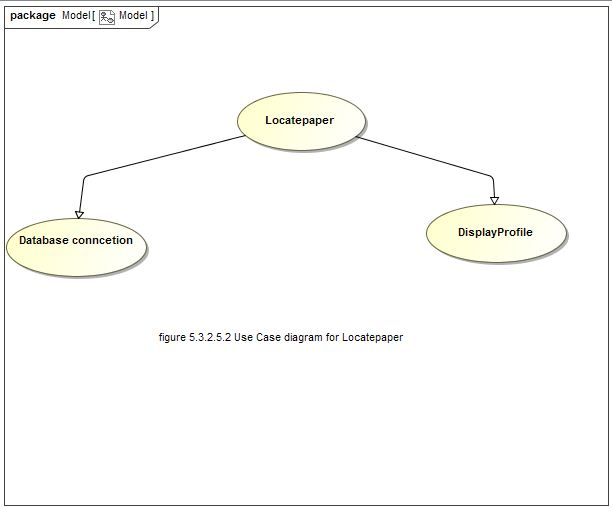
\includegraphics[width=1\textwidth]{./Graphs/UseCaseDiagramforLocatePaper.JPG}\\[0.4cm]
			Figure 5.3.8: Locate Paper
		
		\subsubsection{Manipulate paper} 
		
		This is to provide user (Client browser) to be able to manipulate their current work  	
		
		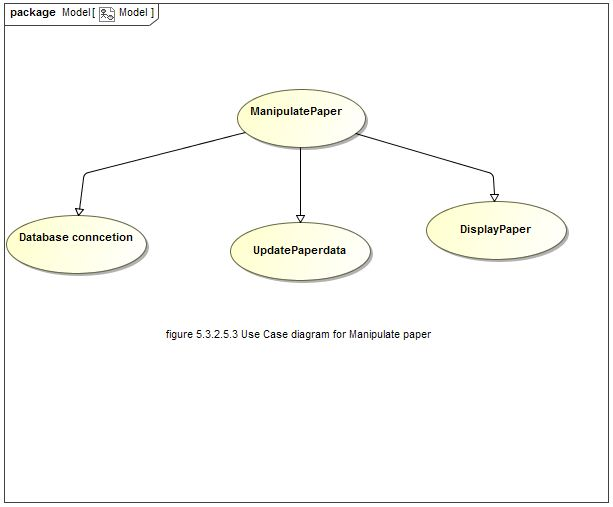
\includegraphics[width=1\textwidth]{./Graphs/UseCaseforManipulatePaper.JPG}\\[0.4cm]
		Figure 5.3.9: Manipulate Paper
		
		
		\subsubsection{View author list}
		
		This is to provide user (Client browser) with the list of authors from the server.
		
		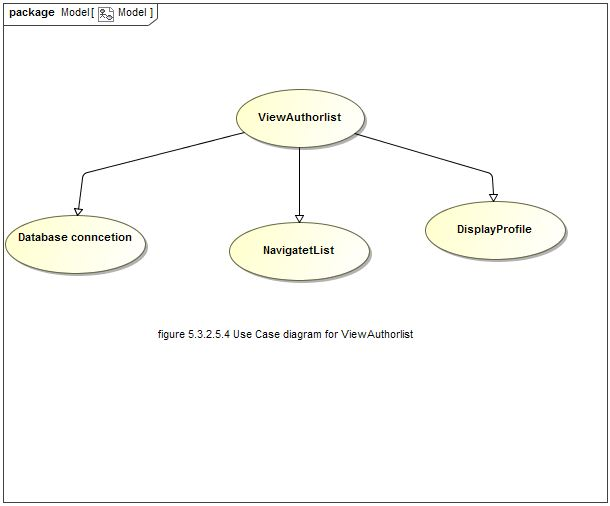
\includegraphics[width=1\textwidth]{./Graphs/UseCasediagramforViewAuthorList.JPG}\\[0.4cm]
		
		
		5.3.10 View Author List
		
		\subsection{Research Portal}
	
		\subsubsection{User Registration}
			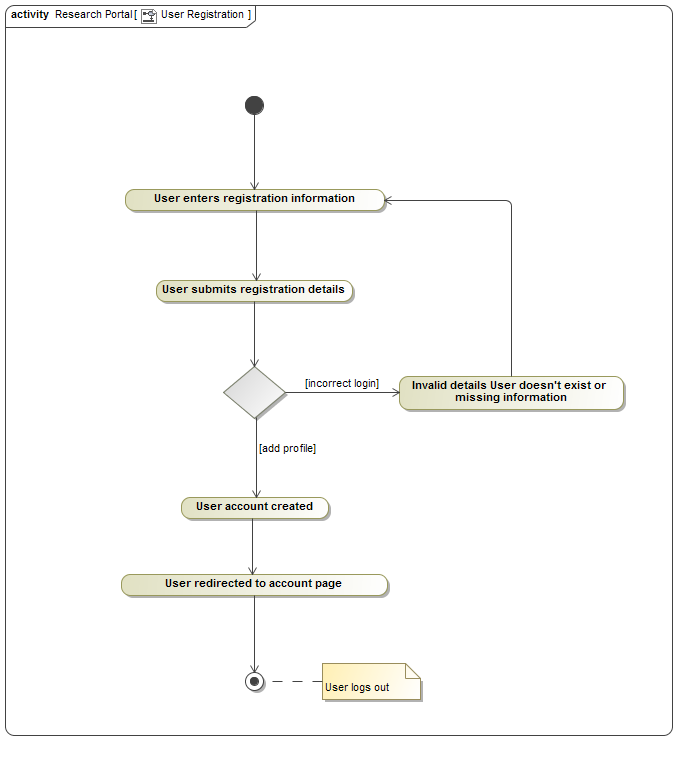
\includegraphics[width=1\textwidth]{./Graphs/UserRegistration.png}\\[0.4cm]
		
		\subsubsection{User Login}
			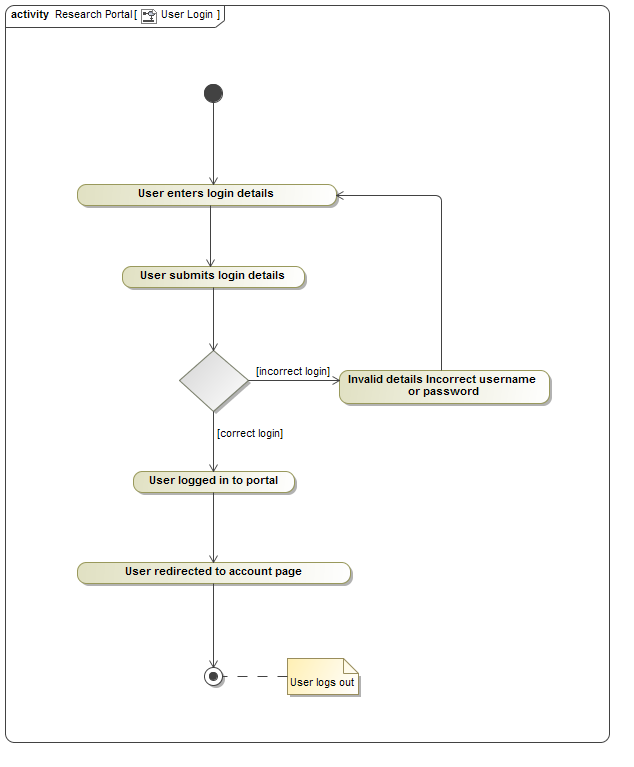
\includegraphics[width=1\textwidth]{./Graphs/UserLogin.png}\\[0.4cm]
			
		\subsubsection{Create/Remove Research Publication}
			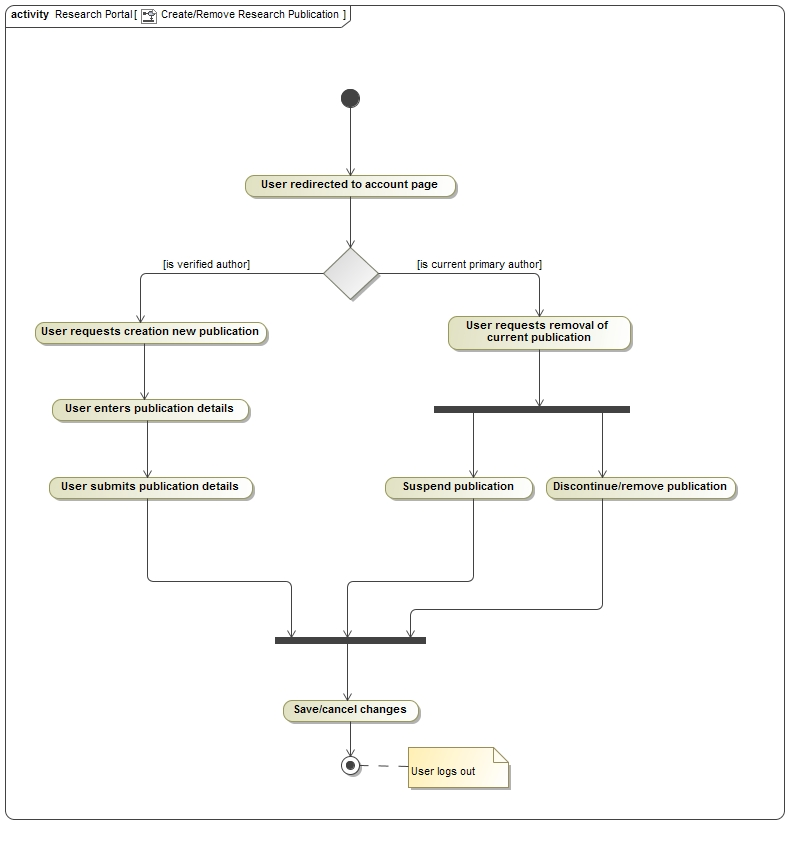
\includegraphics[width=1\textwidth]{./Graphs/CreateRemoveResearchPublication.png}\\[0.4cm]
	
		\subsubsection{View/Modify Research Publication}
		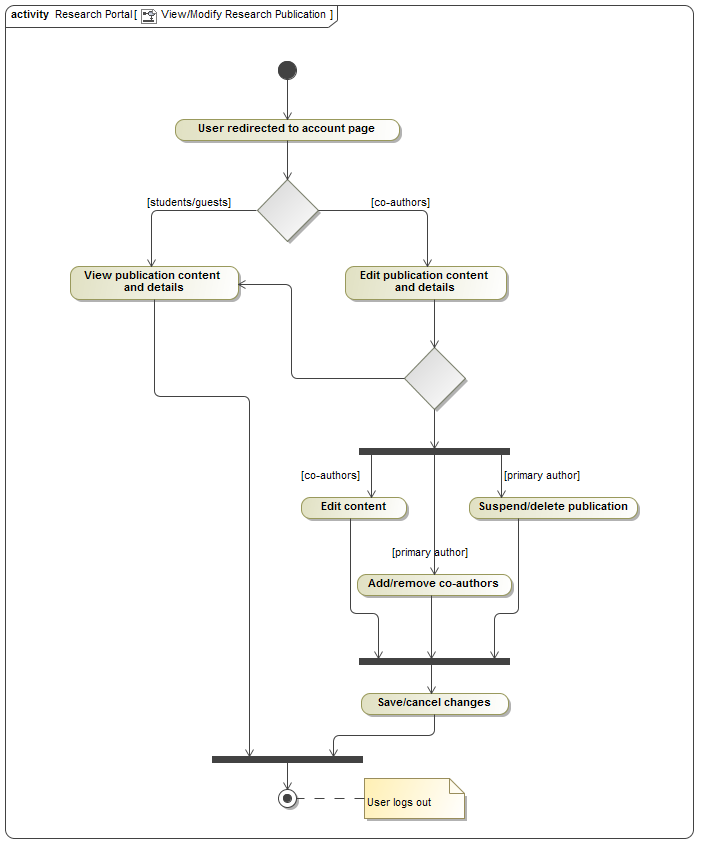
\includegraphics[width=1\textwidth]{./Graphs/ViewModifyResearchPublication.png}\\[0.4cm]
		
		
		\subsection{Domain Model}
		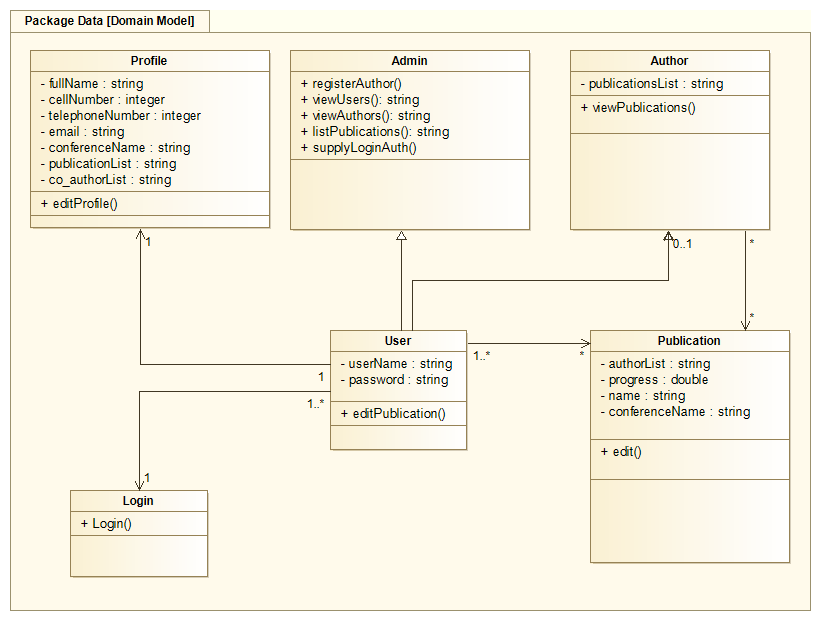
\includegraphics[width=1\textwidth]{./Graphs/DomainModel.png}\\[0.4cm]
	
	\section{Open Issues}
	\begin{itemize}
		\item User name of the client(Client browser)
		\item User password of the Client (Client browser)
		\item Validate with users in database. 
	\end{itemize}
	
	
	
	%\bibliographystyle{IEEEtran}
	%\bibliography{./assignment}
	
\end{document}
